%%
%% This is file `sample-sigconf.tex',
%% generated with the docstrip utility.
%%
%% The original source files were:
%%
%% samples.dtx  (with options: `sigconf')
%%
%% IMPORTANT NOTICE:
%%
%% For the copyright see the source file.
%%
%% Any modified versions of this file must be renamed
%% with new filenames distinct from sample-sigconf.tex.
%%
%% For distribution of the original source see the terms
%% for copying and modification in the file samples.dtx.
%%
%% This generated file may be distributed as long as the
%% original source files, as listed above, are part of the
%% same distribution. (The sources need not necessarily be
%% in the same archive or directory.)
%%
%% The first command in your LaTeX source must be the \documentclass command.
\documentclass[sigconf]{acmart}

%%
%% \BibTeX command to typeset BibTeX logo in the docs
\AtBeginDocument{%
  \providecommand\BibTeX{{%
    \normalfont B\kern-0.5em{\scshape i\kern-0.25em b}\kern-0.8em\TeX}}}

\usepackage{graphicx,url}
\usepackage[utf8]{inputenc}
\usepackage[brazil]{babel}
\usepackage{gensymb}

%% Rights management information.  This information is sent to you
%% when you complete the rights form.  These commands have SAMPLE
%% values in them; it is your responsibility as an author to replace
%% the commands and values with those provided to you when you
%% complete the rights form.
\setcopyright{acmcopyright}
\copyrightyear{2018}
\acmYear{2018}
\acmDOI{10.1145/1122445.1122456}

%% These commands are for a PROCEEDINGS abstract or paper.
\acmConference[Woodstock '18]{Woodstock '18: ACM Symposium on Neural
  Gaze Detection}{June 03--05, 2018}{Woodstock, NY}
\acmBooktitle{Woodstock '18: ACM Symposium on Neural Gaze Detection,
  June 03--05, 2018, Woodstock, NY}
\acmPrice{15.00}
\acmISBN{978-1-4503-9999-9/18/06}


%%
%% Submission ID.
%% Use this when submitting an article to a sponsored event. You'll
%% receive a unique submission ID from the organizers
%% of the event, and this ID should be used as the parameter to this command.
%%\acmSubmissionID{123-A56-BU3}

%%
%% The majority of ACM publications use numbered citations and
%% references.  The command \citestyle{authoryear} switches to the
%% "author year" style.
%%
%% If you are preparing content for an event
%% sponsored by ACM SIGGRAPH, you must use the "author year" style of
%% citations and references.
%% Uncommenting
%% the next command will enable that style.
%%\citestyle{acmauthoryear}

%%
%% end of the preamble, start of the body of the document source.
\begin{document}

%%
%% The "title" command has an optional parameter,
%% allowing the author to define a "short title" to be used in page headers.
\title{Arquitetura de Video Player para Realidade Virtual em Dispositivos Móveis}

%%
%% The "author" command and its associated commands are used to define
%% the authors and their affiliations.
%% Of note is the shared affiliation of the first two authors, and the
%% "authornote" and "authornotemark" commands
%% used to denote shared contribution to the research.
\author{Adriano M. Gil, Afonso R. Costa Jr, Atacilio C. Cunha, Thiago S. Figueira}
\email{{adriano.gil, afonso.j, a.cunha, t.figueira}@sidia.com}

\affiliation{%
  \institution{Sidia Instituto de Ciência e Tecnologia (SIDIA)}
  % \streetaddress{P.O. Box 1212}
  \city{Manaus}
  \state{AM}
  % \postcode{43017-6221}
}

%%
%% By default, the full list of authors will be used in the page
%% headers. Often, this list is too long, and will overlap
%% other information printed in the page headers. This command allows
%% the author to define a more concise list
%% of authors' names for this purpose.
\renewcommand{\shortauthors}{Trovato and Tobin, et al.}

%%
%% The abstract is a short summary of the work to be presented in the
%% article.
\begin{abstract}
  A clear and well-documented \LaTeX\ document is presented as an
  article formatted for publication by ACM in a conference proceedings
  or journal publication. Based on the ``acmart'' document class, this
  article presents and explains many of the common variations, as well
  as many of the formatting elements an author may use in the
  preparation of the documentation of their work.
\end{abstract}

%%
%% The code below is generated by the tool at http://dl.acm.org/ccs.cfm.
%% Please copy and paste the code instead of the example below.
%%
\begin{CCSXML}
<ccs2012>
<concept>
<concept_id>10011007.10010940.10010971.10010972.10010539</concept_id>
<concept_desc>Software and its engineering~n-tier architectures</concept_desc>
<concept_significance>300</concept_significance>
</concept>
</ccs2012>
\end{CCSXML}

\ccsdesc[500]{Computer systems organization~Embedded systems}
\ccsdesc[300]{Computer systems organization~Redundancy}
\ccsdesc{Computer systems organization~Robotics}
\ccsdesc[100]{Networks~Network reliability}

%%
%% Keywords. The author(s) should pick words that accurately describe
%% the work being presented. Separate the keywords with commas.
\keywords{video player, virtual reality}

%%
%% This command processes the author and affiliation and title
%% information and builds the first part of the formatted document.
\maketitle

\section{Introdução}

%% - Contextualizar VR

A Realidade Virtual possui um grande atrativo pelo sua forma inovadora no consumo de conteúdo. Imersão é sua característica mais marcante, possibilitando aos usuários um profundo envolvimento com objetos e cenários em 3D dentro de um mundo virtual.

%% - Contextualizar VR Headsets e VR Mobile


%% - Falar sobre a importância do consumo de mídias no VR Mobile
Aplicações de Realidade Virtual permitem uma maior discrição e um maior sensação de interação com conteúdo multimídia. Assim, mesmo fotos e vídeos usuais se tornam uma experiência diferenciada para o usuário VR. Muitas aplicações tem por mote funcionar como galeria de mídia dentro do ambiente de realidade virtual, por exemplo, \textit{VR Gallery} da Samsung é uma delas.

%% - Contextualizar ferramentas de desenvolvimento para VR Mobile (Unity, GVRF)
Unity é um motor de jogos WYSIWYG (What You See Is What You Get) \cite{sv2015popolin}, atualmente é a mais ampla ferramenta para o desenvolvimento de aplicações de realidade virtual mobile, presente como motor de criação em 60\% do conteúdo criado para realidades virtual e aumentada, conta com uma comunidade de desenvolvedores presentes em todo o mundo, além de ser utilizada por grandes corporações como Microsoft e Disney. (https://unity3d.com/pt/public-relations)

%% - Proposta: Desenvolver uma arquitetura de alto desempenho de video player para plataformas VR mobile
Este artigo tem por proposta a implementação de uma arquitetura de alto desempenho para video player em plataformas de realidade virtual e aumentada utilizando dispositivos móveis. Para avaliações desempenhos serão feitas comparações entre dois frameworks de renderização: Unity e GVRF.

%% - Estrutura do Artigo
Na seção \ref{sec-relatedworks} analisamos alguns trabalhos que descrevem o uso de video players no contexto de dispositivos móveis e em realidade virtual e aumentada. A metodologia adotada é descrita na seção \ref{sec-methodology}. A arquitetura implementada foi definda na seção \ref{sec-videoplayer-arch}. Resultados são apresentados na seção \ref{sec-results}. Por fim, as conclusões e perspectivas de trabalhos futuros são mencionadas na seção \ref{sec-conclusion}

\section{Trabalhos Relacionados} \label{sec-relatedworks}

% TODO: Ainda confuso - melhorar texto
Consumo de mídia é uma atividade de grande importância para usuários dentro do mundo digital, onde existe uma crescente quantidade de conteúdo a ser consumido. Um trabalho \cite{repo2004users} da década passada já levanta essa demanda por uso de mídia em dispositivos móveis como meio de possibilitar entretenimento, lidar com situações entediantes, compartilhar experiências e conhecimento.

Aplicações podem usar o consumo de mídia como uma forma de implementar uma interação específica com o usuário. Em \cite{hu2018kalgan}, é citado um exemplo de aplicação para aprendizado de idiomas utilizando um Video Player com enfoque maior na visualização e manipulação da linguagem contida na mídia.

%% - Listar trabalhos relacionados a video players para VR Mobile
Em \cite{smolic2009overview} são listadas diferentes codecs que podem ser utilizados na transmissão de vídeos estereoscópicos, onde é reforçada a idéia de que a componente de profundidade pode ser comprimida de diferentes maneiras.

%% - Listar trabalhos que falem sobre o desempenho de video players no mobile

O trabalho \cite{wild2018inaccessibility} cita a necessidade de adequar Video Players para serem acessíveis a pessoas portadoras de necessidades especiais. Segundo o artigo é necessário que o Video Player tenha suporte a legendas, descrição de audio, transcrições de mídia, suporte a modificações de volume e contraste de cor.

%% - Listar trabalhos que falem sobre a renderização de videos no VR
MR360 definido em \cite{rhee2017mr360} propõe uma composição de objetos virtuals 3D durante a execução de um video 360. O video panorâmico é usado tanto como fonte de luz para iluminar os objetos virtuais quanto para compor o pano de fundo a ser renderizado.

%% - Listar trabalhos que lidam com o desenvolvimento de plugins Unity Android
Calory Battle AR desenvolvido por \cite{kim2014using} é um jogo de realidade aumentada construído em Unity cujo objetivo é conscientizar o jovem público-alvo sobre os benefícios da alimentação saudável através do estímulo à pratica de exercícios ao explorar o espaço físico em busca do desarmamento das "bombas calóricas".
\cite{sv2015popolin} mostra o desenvolvimento do \textit{Unity Cluster Package}, voltado para a criação de aplicações de multiprojeção para sistemas baseados em Aglomerado Gráfico (AG) através do modelo Mestre-Escravo no editor Unity.

%% - Referenciar nosso trabalho do SVR sobre o GVRF

\section{Metodologia} \label{sec-methodology}

%% - Definir tipos de mídias a serem consumidas no VR Mobile
%% - Definir formas de visualização do conteúdo
%% - Comparativo de diferentes implementações (Unity x GVRF)

Em um ambiente virtual, poderemos ter a manipulação de alguns tipos de mídia, tais como: áudio, imagem e vídeo. Dentre estes, a mídia no formato de vídeo foi escolhida para ser o objeto de estudo deste trabalho. Logo, queremos propor uma arquitetura que tenha um ótimo desempenho em uma plataforma VR no ambiente \textit{mobile}.

Assim, a metodologia pode ser dividida nos seguintes passos:

\begin{enumerate}
    \item Definição dos formatos de vídeo a serem experimentados.
    \item Definição das formas de visualização ou renderização do vídeo no ambiente virtual.
    \item Comparativo de duas diferentes implementações no ambiente \textit{mobile}.
\end{enumerate}

Os vídeos escolhidos para experimentar a arquitetura proposta estão no formato MP4, pois é o formato com grande utilização nos dispositivos móveis. Foram escolhidos dois vídeos curtos (sendo um em 360\degree) para que sejam executados até o fim e com isso avaliarmos o desempenho nas plataformas de desenvolvimento escolhidas. É importante salientar que este trabalho não visa comparar a qualidade dos vídeos (por exemplo, tipo de codificação, compressão, etc.).

A renderização do conteúdo do vídeo será visualizada nas seguintes formas: plano e 360\degree.

Visando testar a arquitetura nos dispositivos móveis, duas plataformas de desenvolvimento foram escolhidas: Unity\footnote{https://unity3d.com/} e GVRF\footnote{http://www.gearvrf.org/}. A métrica que será utilizada será a quantidade de \textit{frames} por segundo. A ferramenta chamada \textit{OVR Metrics Tool} \cite{ovrmetrictool} será utilizada para medir e coletar os valores.

Os experimentos serão realizados em dois dispositivos que contenham diferentes configurações de \textit{hardware}.

\section{Arquitetura} \label{sec-videoplayer-arch}

%% - Poderíamos separar em duas camadas: Plataforma e Renderização.

Buscando a implementação otimizada de um Video Player para plataformas de Realidade Virtual móveis, dividimos nossa arquitetura em duas camadas principais:

\begin{enumerate}
    \item Camada de plataforma: implementação nativa para lidar com operações de I/O para consumo e descompressão de mídias.
    \item Camada de renderização: uso de algum framework de renderização para tornar vísivel dentro de um universo virtual 3D o conteúdo extraído da mídia.
\end{enumerate}

Assim, de acordo com a camada de plataforma, diferentes formatos podem ser suportados, e renderizados de diferentes maneiras na camada de renderização. Por exemplo, um arquivo de video 2000x1000 pode ser visualizado como um video 360 distribuido no entorno do usuário poderia na verdade permitir uma resolução horizontal de cerca de 555 pixels dado um \textit{FOV} de 100 graus. A relação entre a resolução do conteúdo, o campo de visão (\textit{FOV}), e quantidade real de pixels disponibilizados é discutida na subseção \ref{sec-arch-subsec-render-layer}.

\begin{figure*}[h!]
    \centerline{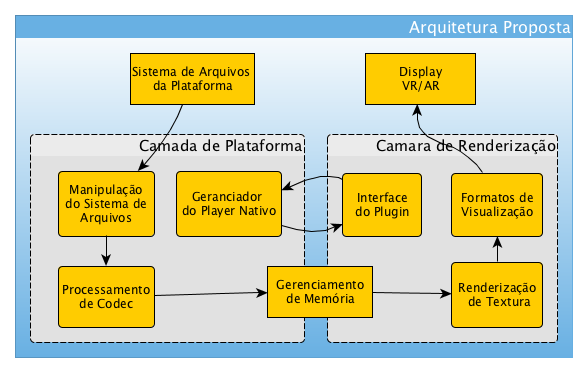
\includegraphics[scale=0.7]{images/video_player_arch_pt}}
    \caption{Arquitera de Video Player proposta}
    \label{fig-video-player-arch}
\end{figure}

Nas subseções a seguir são descritas como as influências da plataforma no consumo do vídeo (subseção \ref{sec-arch-subsec-platform-layer}) e citar algumas possibilidade de renderização permitadas na realidade virtual e aumentada em dispositivos móveis (subseção \ref{sec-arch-subsec-render-layer}).

\subsection{Camada de Plataforma} \label{sec-arch-subsec-platform-layer}

%% - Na questão de Plataforma, descrevemos um pouco o lado do Android de consumo de mídias (Uso do MediaPlayer, MediaCodec, uso do OpenGL, tipos de textura, ….), interação com o Unity via plugins

A camada de plataforma é responsável pelo consumo de mídias, alocação e gerenciamento de memória para armazenar o conteúdo descomprimido, lidar com operações de I/O.

Qualquer aplicação multimídia que execute vídeo precisa não apenas renderizar a mídia digital em um player, mas também necessita de controles que possam ser utilizados por qualquer usuário de maneira que ele possa interagir com este player e também ter informações sobre o status do mesmo.

Na plataforma Android é possível construir um player de vídeo através da classe MediaPlayer e da biblioteca ExoPlayer. A classe MediaPlayer é utilizada para controle básico de reprodução de arquivos de áudio e vídeo. Já a biblioteca ExoPlayer define um padrão de reprodução de áudio e vídeo construídos sobre a utilização da API MediaCodec com features como DASH e HLS não disponíveis na classe MediaPlayer.

A classe MediaCodec oferece diversas possibilidades para o ExoPlayer por oferecer acesso a codecs de mídia em nível baixo de implementação. Isso é possível pois, de maneira simples, os codecs processam dados de entrada para transformar em dados de saída através de diversos buffers de entrada e saída que são processados assincronamente.

MediaCodec trabalha com os seguintes tipos de dados:

\begin{enumerate}
    \item compressed
    \item raw audio
    \item raw video
\end{enumerate}

Qualquer um destes tipos pode ser processado utilizado objetos da classe ByteBuffer, mas para melhorar performance do codec, é necessário usar Surface ao trabalhar com dados do tipo raw video. Isso se dá devido ao uso de buffers nativos onde não se faz necessário o mapeamento ou cópia de dados para objetos ByteBuffers. Vale ressaltar que é inviável acessar dados do tipo raw data quando se utiliza uma Surface, sendo uma solução a utilização de um objeto da classe ImageReader para obter frames de video.

O mimetype de um arquivo define os dados comprimidos dos buffers de entrada e saída. Para vídeos, geralmente é apenas um único frame de vídeo comprimido. Com relação aos buffers de vídeo no modo ByteBuffer, eles são definidos de acordo com o formato de cores que podem ser:

\begin{enumerate}
    \item formato native raw video
    \item buffers YUV flexíveis
    \item outros, de formato específicos: geralmente suportado pelo modo ByteBuffer
\end{enumerate}


Todo codec possui estados que mapeam ações durante seu ciclo de vida. Eles podem assumir os estados Stopped, Executing e Released. O estado Stopped mapeia um conjunto de outros sub-estados que são Unintialized, Configured e Error, enquanto o estado Executing se desenvolve sobre outros sub-estados que são Flushed, Running e End-of-Stream.

O codec ao ser criado por qualquer factory, começa pelo estado Unintialized. Ao ser configurado através da utilização de configure(), passa para Configured e então ao ser chamado start(), o codec passa para o estado Executing, especificamente entrando pelo sub-estado Flushed que onde já se contém todos os buffers. Quando o primeiro buffer sai da fila, o sub-estado do codec passa para Running e quando um buffer com o marcado de end-of-stream é colocado na fila, o codec passa para o estado End of Stream. Se durante a execução do codec o método flush() for executado, ele retorna para o estado Flushed. A chamada stop() retorna ele para o estado Unintialized e raramente quando, durante a execução do codec, há algum erro, o codec passa para o estado Error. Durante qualquer momento, se o método release() for chamado, o codec passa para o estado Released.

É possível criar aplicações Android com alta performance de gráficos 2D e 3D através da API OpenGL ES e também do Native Development Kit (NDK). OpenGL é uma interface de programação que permite comunicação e manipulação de processamento de gráficos 3D no hardware responsável. O Android suporta as seguintes versões da API OpenGL ES:
\begin{enumerate}
    \item OpenGL ES 1.0: Android 1.0+
    \item OpenGL ES 2.0: Android 2.2(API Level 8)+
    \item OpenGL ES 3.0: Android 4.3(API Level 18)+
    \item OpenGL ES 3.1: Android 5.0(API Level 21)+
\end{enumerate}

A manipulação de gráficos através da API OpenGL ES se dá a partir da classe GLSurfaceView e da interface GLSurfaceView.Renderer.
A classe GLSurfaceView é uma View utilizada para desenhar e manipular objetos através de chamadas feitas à API OpenGL ES. Já a interface GLSurfaceView.Renderer é responsável por fazer chamadas OpenGL para renderizar um frame através da especificação dos seguintes métodos que precisam ser implementados:
onSurfaceCreated(): geralmente chamado uma única vez para definição dos parâmetros de ambiente OpenGL que serão utilizados durante a execução ou para inicializar objetos da API;
onDrawFrame(): chamado a cada vez que a GLSurfaceView precisar ser redesenhada;
e onSurfaceChanged(): chamado sempre que a geometria da GLSurfaceView for alterada, incluindo definições de tamanho da GLSurfaceView e orientação da tela do dispositivo.
Dentro deste contexto, uma aplicação comum que utiliza a API OpenGL ES cria diversas texturas durante seu tempo de execução. Sabe-se que texturas em alta resolução ajudam no resultado final da aplicação em alcançar gráficos melhores e muitas vezes até em melhorar a experiência do usuário que utiliza algo dependente deste tipo de tecnologia. Mas quanto maior a resolução, mais memória se demanda para gerenciamento e mais tempo se gasta em carregamento. Um exemplo disso são as extensões JPG e PNG que não são descomprimidos diretamente pela GPU.
Uma forma de melhorar a performance da aplicação, consumo de bateria, aquecimento do dispositivo e até mesmo diminuir muitas vezes o tamanho das APK's geradas é fazer uso dos formatos hardware accelerated. Para este formato, há duas categorias: as padrões e as proprietárias.

Os formatos padrões para trabalhar com texturas hardware accelerated são:

\begin{enumerate}
    \item ETC1: suportado em todos o dispositivos com OpenGL ES 2.0+
    \item ETC2: suportado nos dispositivos com OpenGL ES 3.0+
    \item ASTC: Suportado com Android Extension Pack.
\end{enumerate}

Já os formatos proprietários são os seguintes:

\begin{enumerate}
    \item ATC: disponível em Adreno GPU
    \item PVRTC: disponível em PowerVR GPU
    \item DXT1 e S3TC: disponível em dispositivos Nvidia Tegra Platform
\end{enumerate}

Com base em vários formatos, é preciso avaliar qual atende melhor a necessidade da aplicação que está sendo desenvolvida, mas o melhor caso é quando o Android Extension Pack é suportado. Neste Pack está disponível o formato de compressão ATSC (Adaptive Scalable Texture Compreension), definido neste como padrão e, desta forma, exclui a necessidade de trabalhar com tipos diferentes para plataformas diferentes. Atualmente o ATSC possui qualidade maior que outros formatos disponíveis na GPU por ter suporte alfa completo e melhor conservação da qualidade.

% Texturas de vídeo (Surface, Texturas OES): Falar que videos normalmente são renderizados em texturas do tipo OES.
Uma das partes menos documentadas na literatura é a renderização em texturas. A utilização de texturas permite a atualização e renderização contínua de componentes dinâmicos como sites, vídeos e outros. Para objetos estáticos, a melhor abordagem é trabalhar com bitmap.

A funcionamento de texturas de vídeos dependem de alguns passos. Primeiramente, é importante criar uma classe que implemente a interface GLSurfaceView.Renderer e em tal classe é definida a especificação da atualização de textura por frame. As texturas utilizadas para vídeo possuem seus canvas atualizados dentro do método executado pela thread GL que gerencia esta etapa. No Android, na maioria das vezes se trata de um método onDraw() do componente. O ponto principal da definição das texturas que são criadas com este objetivo é sua definição como $GL_TEXTURE_EXTERNAL_OES$ ao invés de $GL_TEXTURE_2D$. Isto se dá pois as texturas do tipo OES possuem uma tabela de textura semi-global na GPU que permite que elas seja utilizadas em outros contextos GL, garantindo assim segurança na sua utilização.

\subsection{Camada de Renderização} \label{sec-arch-subsec-render-layer}

A camada de renderização é responsável explorar diferentes formas de visualização do video, seja em um plano, numa esfera em 360, em um grid de voxels, utilizando os mais diversos shaders...

%% - Na Renderização podemos

\subsubsection{Renderização de Vídeo usando Unity}

%% - Mencionar StateMachines

Unity é...


\subsubsection{Renderização de Vídeo usando GVRF}

% TO REPHRASE
\textit{GearVR framework} (GVRf) é fornecido como uma biblioteca de APIs para renderização de aplicações VR/AR/MR. Sua sintaxe de código traça similaridades com as \textit{APIs} de motores gráficos de jogos, por exemplo, fornecendo uma \textit{pipeline} conhecida a maioria dos desenvolvedores de jogos: e.g, objetos do mundo 3D se organizam em cenas e também podem ter suas visualizações configuradas por materiais, estes que podem possuir seus próprios \textit{shaders}, código destinados a GPU com instruções para a renderização de cada pixel pertecente ao objeto alvo.


\section{Resultados} \label{sec-results}

%% - A idéia é apresentar como resultado uma curta análise de desempenho (medidas de FPS, ….) de uma ou mais aplicações rodando esse video player.
%% - Comparar GVRF x Unity

Lorem ipsum dolor sit amet, consectetur adipisicing elit, sed do eiusmod
tempor incididunt ut labore et dolore magna aliqua. Ut enim ad minim veniam,
quis nostrud exercitation ullamco laboris nisi ut aliquip ex ea commodo
consequat. Duis aute irure dolor in reprehenderit in voluptate velit esse
cillum dolore eu fugiat nulla pariatur. Excepteur sint occaecat cupidatat non
proident, sunt in culpa qui officia deserunt mollit anim id est laborum.

\section{Conclusão e Trabalhos Futuros} \label{sec-conclusion}

%% - Podemos mencionar a necessidade de mensurar o real desempenho da execução/rasterização do vídeo, puxando assim o gancho para o próximo paper.

Lorem ipsum dolor sit amet, consectetur adipisicing elit, sed do eiusmod
tempor incididunt ut labore et dolore magna aliqua. Ut enim ad minim veniam,
quis nostrud exercitation ullamco laboris nisi ut aliquip ex ea commodo
consequat. Duis aute irure dolor in reprehenderit in voluptate velit esse
cillum dolore eu fugiat nulla pariatur. Excepteur sint occaecat cupidatat non
proident, sunt in culpa qui officia deserunt mollit anim id est laborum.

%%
%% The acknowledgments section is defined using the "acks" environment
%% (and NOT an unnumbered section). This ensures the proper
%% identification of the section in the article metadata, and the
%% consistent spelling of the heading.
\begin{acks}
To Robert, for the bagels and explaining CMYK and color spaces.

Identification of funding sources and other support, and thanks to
individuals and groups that assisted in the research and the
preparation of the work should be included in an acknowledgment
section, which is placed just before the reference section in your
document.
\end{acks}

%%
%% The next two lines define the bibliography style to be used, and
%% the bibliography file.
\bibliographystyle{ACM-Reference-Format}
\bibliography{video_player_arch}

%%
%% If your work has an appendix, this is the place to put it.
% \appendix

\end{document}
\endinput
%%
%% End of file `sample-sigconf.tex'.
